\documentclass[11pt,a4paper]{article}

\usepackage[utf8]{inputenc}
\usepackage[T1]{fontenc}
\usepackage[spanish]{babel}

\usepackage{tgpagella}
\usepackage{geometry}
\usepackage{booktabs}
\usepackage{xcolor}
\usepackage{graphicx}
\usepackage{titlesec}
\usepackage{fancyhdr}
\usepackage[parfill]{parskip}
\usepackage[expansion=false]{microtype}
\usepackage{hyperref}
\usepackage{setspace}
\usepackage{needspace}
\usepackage{etoolbox}
\usepackage{ragged2e}

\widowpenalty=10000
\clubpenalty=10000
\displaywidowpenalty=10000

\hyphenpenalty=8000
\exhyphenpenalty=8000

\geometry{top=3.0cm,bottom=3.0cm,left=3.5cm,right=3.5cm}

\setlength{\parskip}{0.65em}
\setlength{\parindent}{0em}

\definecolor{azulai}{RGB}{30,80,140}
\definecolor{doradoai}{RGB}{140,90,0}
\definecolor{grisai}{RGB}{70,70,70}

\AtBeginDocument{\justifying}

\titleformat{\section}
{\Large\bfseries\color{azulai}\justifying}
{}
{0em}
{}
[{\color{azulai}\titlerule[0.5pt]}]

\titlespacing*{\section}
{0pt}{1.3em}{0.5em}

\titleformat{\subsection}
{\large\bfseries\color{doradoai}\justifying}
{}
{0em}
{}

\titlespacing*{\subsection}
{0pt}{1.0em}{0.35em}

\titleformat{\subsubsection}
{\normalsize\bfseries\color{grisai}\justifying}
{}
{0em}
{}

\titlespacing*{\subsubsection}
{0pt}{0.8em}{0.25em}

\preto\section{\Needspace{8\baselineskip}}
\preto\subsection{\Needspace{6\baselineskip}}
\preto\subsubsection{\Needspace{4\baselineskip}}

\pagestyle{fancy}
\fancyhf{}

\rhead{\textcolor{grisai}{\small Amaya Beatriz — Arquitectura Interna}}
\lhead{\textcolor{grisai}{\small Mercurio · Venus · Marte}}
\cfoot{\textcolor{grisai}{\small\thepage}}

\renewcommand{\headrulewidth}{0.3pt}

\hypersetup{
colorlinks=true,
linkcolor=azulai,
urlcolor=azulai
}

\setstretch{1.32}

\tolerance=1500
\emergencystretch=4em

\begin{document}

% ── Portada ──────────────────────────────────────────────────────────────────

\begin{titlepage}
  \centering

  \vspace*{2cm}

  {\Huge\bfseries\color{azulai} Mercurio · Venus · Marte}\\[0.6cm]

  {\large\color{grisai} Arquitectura Interna}\\[0.4cm]

  {\small\itshape\color{grisai}
  Procesamiento, vínculo y acción en el funcionamiento cotidiano
  }\\[2.2cm]

  {\huge\color{doradoai} Amaya Beatriz}\\[1.6cm]

  {\Large 30/10/1976 \quad 22:10}\\[0.35cm]

  {\Large Zaragoza, España}\\[0.35cm]

  {\normalsize
  Lat: 41.6916° \quad
  Lon: -0.9101° \quad
  UTC+01:00
  }\\[0.35cm]

  {\normalsize
  Ascendente: Cáncer 16°08'
  \quad
  MC: Piscis 25°32'
  }\\[2.2cm]

  \renewcommand{\arraystretch}{1.35}

  \begin{tabular}{ll}
    \textbf{Mercurio:} & Escorpio — Casa 5 2°48' \\
    \textbf{Venus:}    & Sagitario — Casa 6 12°22' \\
    \textbf{Marte:}    & Escorpio — Casa 5 15°07' \\
  \end{tabular}

  \vfill

  {\small\color{grisai}
  Generado el 20/05/2026
  }

\end{titlepage}

\justifying

\tableofcontents

\clearpage

% ── Datos de referencia ───────────────────────────────────────────────────────
\section{Datos de referencia}

\begin{center}
\renewcommand{\arraystretch}{1.25}
\begin{tabular}{llll}
  \toprule
  \textbf{Planeta} & \textbf{Signo} & \textbf{Casa} & \textbf{Posición} \\
  \midrule
  Mercurio  & Escorpio  & 5  & 2°48' \\
  Venus    & Sagitario & 6 & 12°22' \\
  Marte    & Escorpio & 5 & 15°07' \\
  Ascendente          & Cáncer           & ---                    & 16°08' \\
  Medio Cielo         & Piscis            & ---                    & 25°32' \\
  \bottomrule
\end{tabular}
\end{center}
\justifying

\vspace{0.5cm}

\textbf{Aspectos entre planetas personales:}

\vspace{0.3cm}\textit{No hay aspectos entre los planetas personales en los orbes definidos.}

\justifying

\vspace{0.7cm}

\begin{center}
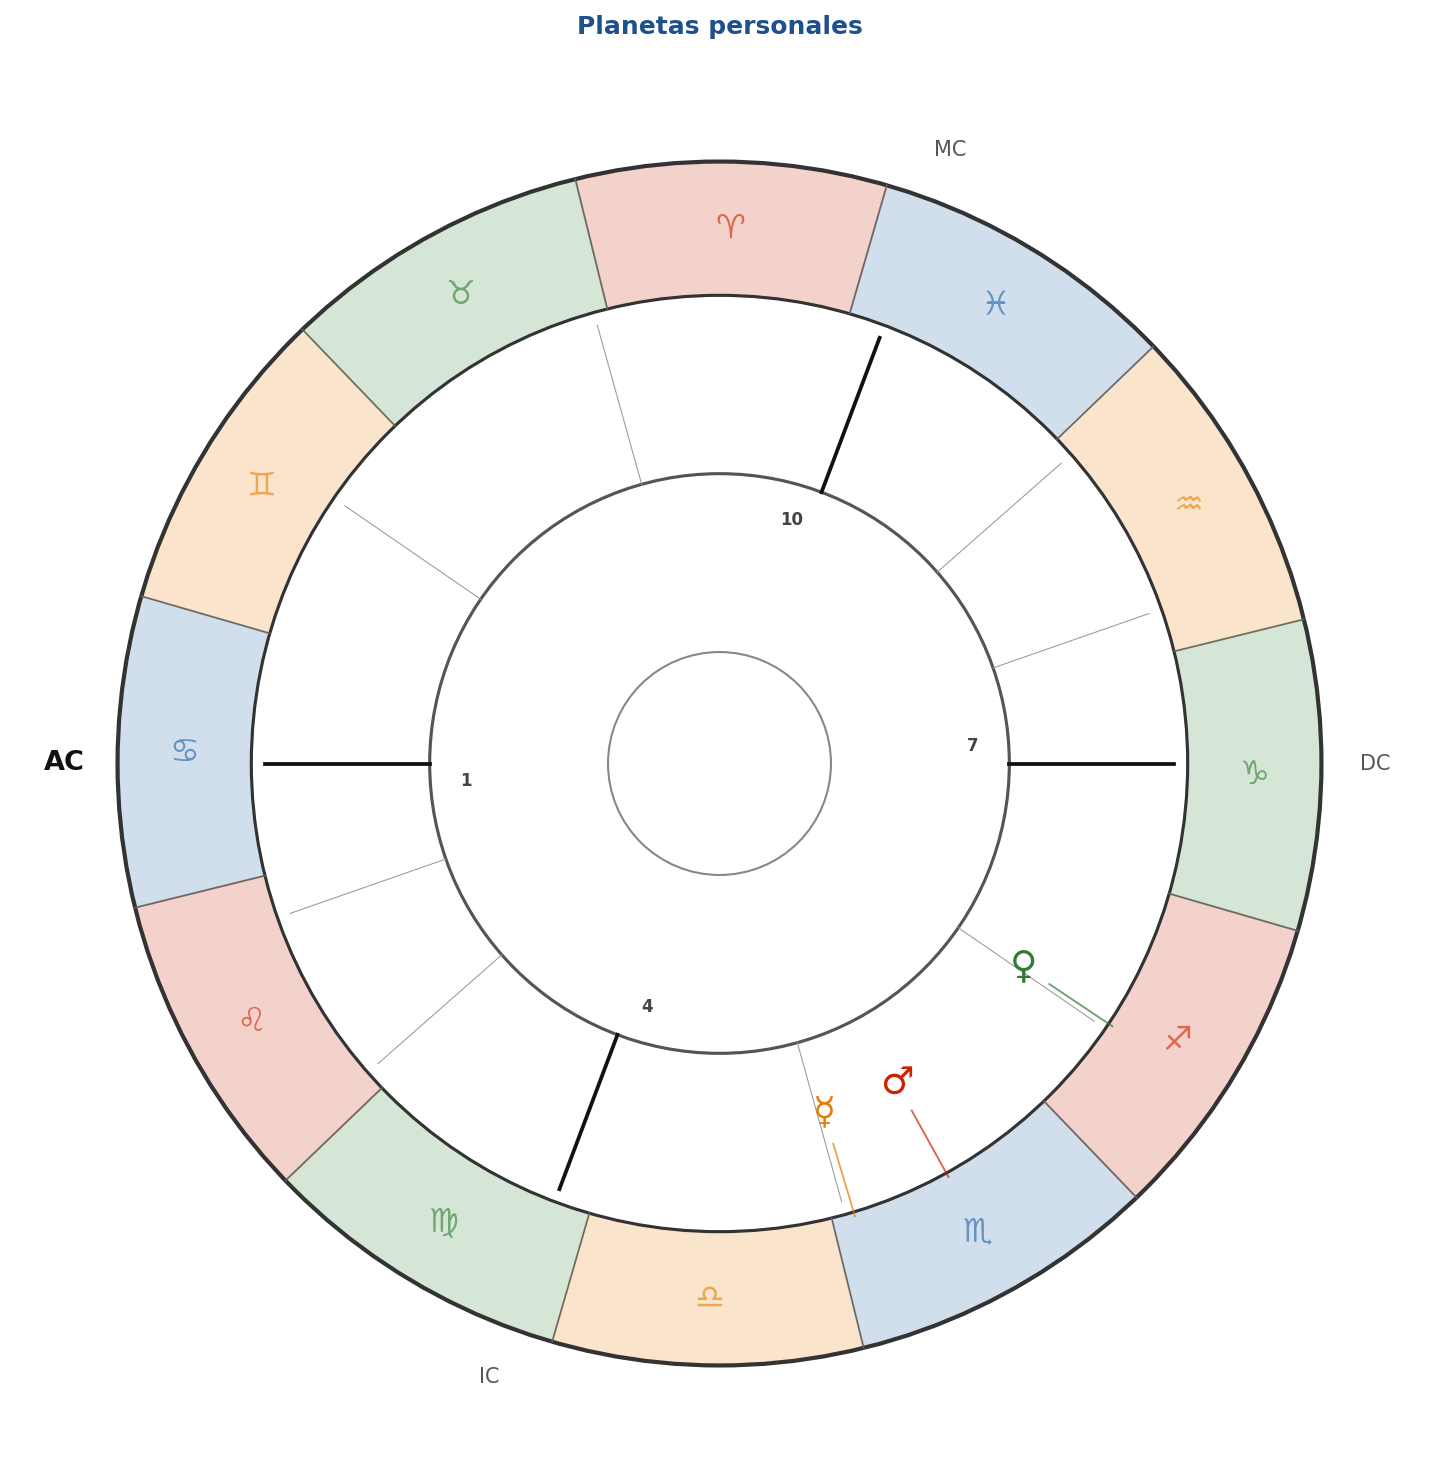
\includegraphics[width=0.72\textwidth]{Amaya_Beatriz_Planetas_Personales_rueda.png}
\end{center}

\vspace{0.3cm}
\Needspace{5\baselineskip}

% ── Interpretación ────────────────────────────────────────────────────────────
\section{Interpretación — Arquitectura Interna}

\begin{center}
{\small\itshape\color{grisai}
No se trata de describir la personalidad.\\
Se trata de observar cómo procesas, cómo te vinculas\\
y cómo se mueve tu energía en la vida cotidiana.
}
\end{center}

\justifying

\vspace{0.8cm}

% ── 1. Funcionamiento general ─────────────────────────────────────────────────
\subsection{1. Funcionamiento general}

\justifying
Mercurio está en Escorpio, Casa 5: muestra cómo piensas, cómo ordenas lo que percibes y cómo traduces lo que ocurre en palabras o ideas.
Venus está en Sagitario, Casa 6: muestra cómo te vinculas, qué necesitas para sentir conexión y cómo buscas equilibrio afectivo.
Marte está en Escorpio, Casa 5: muestra cómo se activa tu acción, cómo descargas energía y cómo respondes ante el impulso.

Hay una concentración funcional entre Mercurio, Marte. Estas dos áreas tienden a activarse de forma cercana. Cuando una se mueve, la otra suele implicarse también. Esto puede dar fluidez, pero también puede hacer que cueste separarlas bajo presión.

Hay coherencia elemental entre: tu forma de pensar (Mercurio) y tu forma de actuar (Marte) comparten elemento: Agua. Esto facilita que esas áreas colaboren entre sí. Aun así, lo que fluye con facilidad también puede volverse automático si no lo observas con consciencia.

Hay tensión elemental entre: tu forma de pensar (Mercurio, Agua) y tu forma de vincularte (Venus, Fuego); tu forma de vincularte (Venus, Fuego) y tu forma de actuar (Marte, Agua). Esto no es un problema en sí mismo, pero sí pide más atención. Cuando esas áreas necesitan cooperar, conviene hacer una integración consciente para que una no bloquee, desborde o desconecte a la otra.

No aparecen aspectos clásicos entre los planetas personales dentro de los orbes definidos. Aun así, puede existir una concentración funcional si los planetas están próximos por signo, por casa o por continuidad de experiencia.

\vspace{0.8cm}

% ── 2. Mercurio ───────────────────────────────────────────────────────────────
\subsection{2. Mercurio — Pensamiento y procesamiento}

\subsubsection*{Mercurio en Escorpio — Casa 5}

\justifying
Tu mente busca profundidad y coherencia. Percibes rápidamente lo que parece ambiguo, incompleto o poco auténtico y tiendes a investigar lo que hay debajo de la superficie.

La saturación aparece cuando percibes contradicciones que no puedes verificar. Entonces tu mente queda atrapada intentando entender qué falta o qué no encaja. El bloqueo suele aparecer como silencio o reserva: cuando algo no puede expresarse con suficiente verdad o profundidad, prefieres no decir nada.

Sueles pensar mejor cuando hay privacidad, claridad emocional y espacios donde no te sientes expueste.

Necesitas creatividad, expresión y participación personal para activar la mente. Comprendes mejor cuando puedes jugar con las ideas, explicarlas a tu manera o transformarlas en algo creativo y vivo.

La saturación aparece cuando el pensamiento se vuelve excesivamente rígido, repetitivo o limitado a tareas puramente técnicas. Entonces disminuye el interés y la atención pierde vitalidad. Sueles regularte mejor cuando puedes crear, enseñar, explicar o expresarte de forma más libre.

\vspace{0.8cm}

% ── 3. Venus ──────────────────────────────────────────────────────────────────
\subsection{3. Venus — Vínculo y regulación relacional}

\subsubsection*{Venus en Sagitario — Casa 6}

\justifying
Necesitas libertad, crecimiento y sensación de expansión compartida dentro del vínculo. La relación suele fortalecerse cuando permite explorar, aprender y mantener espacios propios además de los compartidos.

La saturación aparece cuando la relación se vive como limitación, exceso de control o rutina demasiado cerrada. Entonces la energía afectiva empieza a alejarse incluso antes de que exista conflicto abierto. Cuando el vínculo deja de sostenerse, tiendes a tomar distancia rápidamente para recuperar amplitud y movimiento.

Sueles regularte mejor en relaciones donde existe honestidad, movimiento y suficiente libertad para seguir creciendo.

Necesitas cuidado concreto y presencia cotidiana para sostener el vínculo. Muchas veces expresas el afecto mediante pequeños actos, ayuda mutua y atención práctica a las necesidades de la otra persona.

La saturación aparece cuando la relación se convierte únicamente en responsabilidad o cuando el cuidado deja de ser recíproco. Entonces el vínculo empieza a sentirse más como obligación que como conexión real. Sueles regularte mejor mediante rutinas simples, cooperación y gestos cotidianos de cuidado mutuo.

\vspace{0.8cm}

% ── 4. Marte ──────────────────────────────────────────────────────────────────
\subsection{4. Marte — Acción y descarga}

\subsubsection*{Marte en Escorpio — Casa 5}

\justifying
Tu energía se activa con intensidad y concentración. Respondes con mucha fuerza cuando percibes amenaza, desafío o necesidad de transformación profunda. La acción descarga mediante enfoque, confrontación o procesos de cambio radical.

La saturación aparece cuando la energía queda acumulada sin salida clara. Entonces puedes entrar en estados de control excesivo, obsesión o activación interna permanente. La tensión retenida durante mucho tiempo puede descargarse de forma muy intensa cuando finalmente encuentra salida.

Sueles regularte mejor mediante actividad intensa, profundidad emocional y espacios donde puedas actuar con honestidad y enfoque.

Necesitas creatividad, juego y expresión activa para que tu energía circule bien. Descargas mediante deporte, sexualidad, placer físico o actividades donde puedas implicarte con intensidad y disfrute.

La saturación aparece cuando toda tu energía queda reducida a obligación, rutina o exceso de control. Entonces disminuye la vitalidad y aparece frustración acumulada. Sueles regularte mejor mediante movimiento creativo, juego y experiencias donde puedas expresarte libremente.

\vspace{0.8cm}

% ── 5. Integración ────────────────────────────────────────────────────────────
\subsection{5. Integración — Coherencias, fricciones y bucles}

\justifying
Hay una integración fuerte entre Mercurio, Marte. Estas áreas se activan de manera cercana y conviene observarlas juntas. A veces una de ellas expresa la tensión que en realidad empezó en la otra.

Mercurio (Escorpio, Agua) y Venus (Sagitario, Fuego) operan en elementos que crean tensión. Lo que necesitas para procesar y lo que necesitas para vincularte no siempre siguen la misma lógica.

Mercurio y Marte comparten elemento en Agua. El pensamiento puede convertirse en acción sin demasiada fricción. La facilidad está en pasar de la idea al movimiento; la observación necesaria está en no actuar automáticamente sin verificar.

Venus (Sagitario, Fuego) y Marte (Escorpio, Agua) operan en elementos que crean tensión. Lo que necesitas para conectar y lo que necesitas para actuar no siempre se refuerzan. Cuando hay demanda simultánea de vínculo y acción, puedes tender a priorizar una cosa a expensas de la otra.

Cuando hay demasiada presión, puede aparecer una cadena reconocible: Mercurio en Escorpio queda atrapado repasando lo que no ha terminado de procesar emocionalmente. Desde ahí, Venus en Sagitario se aleja del vínculo o usa la relación como escenario de descarga. Y Marte en Escorpio se disipa o actúa en dirección del entorno antes que desde el propio impulso. El ciclo se cierra cuando la energía acumulada vuelve a saturar el punto inicial.

\vspace{0.8cm}

% ── 6. Orientación práctica ───────────────────────────────────────────────────
\subsection{6. Orientación práctica}

\subsubsection*{Desde dónde empezar}

\justifying
Desde tu forma de vincularte (Venus) en Sagitario, Casa 6. De las tres áreas, esta suele requerir menos energía para activarse. La entrada es activar el movimiento antes de intentar resolverlo todo mentalmente. Empezar por aquí puede abrir movimiento en el resto.

\subsubsection*{Qué sostener}

\justifying
Conviene sostener especialmente tu forma de pensar (Mercurio) en Escorpio: tiempo de integración, silencio emocional y límites sensibles. Bajo presión, esta área puede desorganizarse antes que las demás. Cuando se estabiliza, el resto de tu funcionamiento tiene más capacidad para reorganizarse.

\subsubsection*{Qué evitar}

\justifying
Evitar asumir que la ausencia de fricción visible significa que todo está bien. A veces los bucles no hacen ruido porque te has acostumbrado a funcionar así.

\vspace{0.6cm}

\justifying
Si no se sostiene: pensamiento, vínculo y acción empiezan a funcionar por separado. Lo que piensas no alimenta la acción, la acción no informa al vínculo y el vínculo no regula la energía disponible. El esfuerzo aumenta, la claridad disminuye y la saturación llega antes.

\vspace{1.2cm}

\begin{center}
{\small\itshape\color{grisai}
La astrología se utiliza aquí como lenguaje simbólico de observación,\\
no como una definición cerrada de quién eres.\\[0.2cm]
Este documento propone una lectura funcional y orientativa, no un diagnóstico.
}
\end{center}

\end{document}
